\scanpage{133}
% archive sheet number: 132
\figure{\begin{tikzpicture}[scale=.72]
\foreach \x in {0,1.5,3.3}{\fill (\x,.34) circle (2.25pt) (\x+.77,.34) circle (2.25pt);\draw (\x-.06,.13).. controls (\x+.14,-.03) and (\x+.28,.23)..(\x+.42,.04)..controls(\x+.58,.14) and (\x+.63,.1)..(\x+.82,.15);}
\draw (6.45,-.22)--(7.1,.36)--(7.51,-.64)--cycle (7.57,-.75)--(8.45,-.69)--(8.49,-1.59)--cycle;
\fill (8.49,-1.59) circle(2.2pt);
\end{tikzpicture}}
\[
\lambda_{12}
\]
\figure{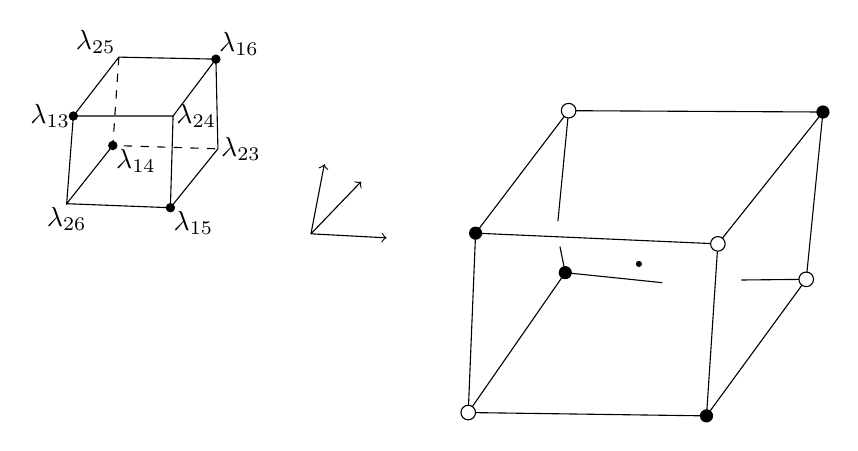
\begin{tikzpicture}[scale=.85,every node/.style={inner sep=1pt}]
\coordinate (a) at (0,0);\coordinate (b) at (1.55,-.06);\coordinate (c) at (2.26,.82);\coordinate (d) at (.69,.87);
\coordinate (e) at (.1,1.31);\coordinate (f) at (1.59,1.31);\coordinate (g) at (2.23,2.16);\coordinate (h) at (.78,2.19);
\draw (a)--(b)--(c)--(g)--(h)--(e)--(a)--(d) (e)--(f)--(g) (b)--(f);
\draw[dashed] (h)--(d)--(c);
\foreach \p in {e,b,d,g}{\fill (\p) circle(2pt);}
\node[below] at (a){$\lambda_{26}$};\node[below right] at (b){$\lambda_{15}$};\node[right] at (c){$\lambda_{23}$};\node[below right] at (d){$\lambda_{14}$};
\node[left] at (e){$\lambda_{13}$};\node[right] at (f){$\lambda_{24}$};\node[above right] at (g){$\lambda_{16}$};\node[above left] at (h){$\lambda_{25}$};
\begin{scope}[xshift=3.65cm,yshift=-.45cm]
\draw[->] (0,0)--(.2,1.04);\draw[->] (0,0)--(.75,.78);\draw[->] (0,0)--(1.13,-.06);
\end{scope}
\begin{scope}[xshift=6cm,yshift=-3.12cm]
\coordinate (a) at (0,0);\coordinate (b) at (3.56,-.05);\coordinate (c) at (5.05,1.99);\coordinate (d) at (1.45,2.09);
\coordinate (e) at (.11,2.68);\coordinate (f) at (3.73,2.52);\coordinate (g) at (5.3,4.49);\coordinate (h) at (1.5,4.51);
\draw (a)--(b)--(c)--(g)--(h)--(e)--(a)--(d) (e)--(f)--(g) (b)--(f) (h)--(1.34,2.86) (1.37,2.48)--(d)--(2.9,1.94) (4.08,1.98)--(c);
\foreach \p in {a,c,f,h}{\draw[fill=white] (\p) circle(3.1pt);}
\foreach \p in {b,d,e,g}{\fill (\p) circle(2.8pt);}
\fill (2.55,2.22) circle(1.3pt);
\end{scope}
\end{tikzpicture}}
\[
\lambda_{12}\left\{\begin{aligned}
&\lambda_{46},\lambda_{35}\\
&\lambda_{34},\lambda_{56}\\
&\lambda_{45},\lambda_{36}
\end{aligned}\right.
\]
\[
e_1+e_2/e_2+e_3/e_3+e_1
\]
\diagram{\begin{tikzcd}[ampersand replacement=\&,row sep=small]
\text{cube}\arrow[r,leftrightarrow]\&\text{cour ponctuée}\\
(\mathrm{Ens})_{2,2,2}\&(\mathrm{Ens})_2\times(\mathrm{Ens})_4\\
\unsure{\mathfrak S|\mathcal S|\mathcal G}_3.(\pm1)^3\arrow[r,phantom,"\simeq"]\&\mathfrak S_2\times\mathfrak S_4
\end{tikzcd}}
\figure{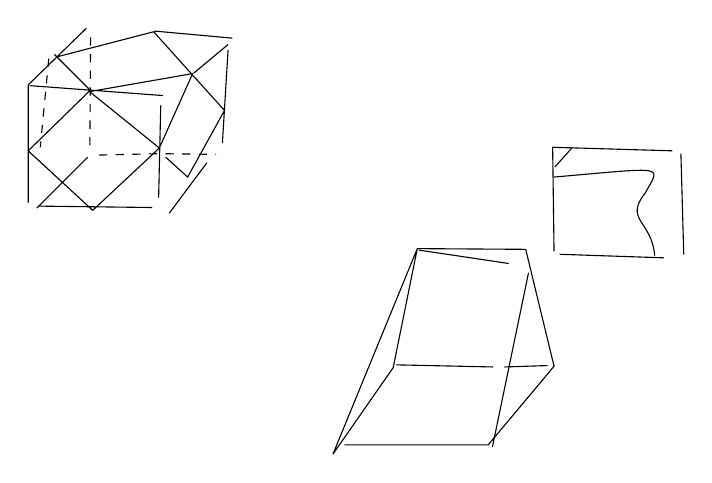
\begin{tikzpicture}[scale=.9]
\draw (0,.07)--(0,1.73)--(.82,2.53) (.02,1.72)--(1.9,1.58) (0,.8)--(.86,1.64)--(1.85,.84)--(.91,-.04)--(0,.8) (.14,.02)--(1.75,.0) (1.84,.14)--(1.87,1.44) (.37,2.16)--(.89,1.64)--(2.32,1.89)--(1.85,.84) (.42,2.13)--(1.77,2.48)--(2.3,1.89)--(2.77,1.37)--(2.25,.43)--(1.94,.71) (1.78,2.49)--(2.88,2.39) (2.34,1.9)--(2.82,2.3) (2.82,2.22)--(2.74,.91) (2.52,.63)--(1.99,-.08) (.12,-.01)--(.84,.71);
\draw[dashed,thin] (.29,2.1)--(.17,.85) (.88,2.4)--(.87,.85) (1.0,.74)--(1.85,.76)--(2.65,.75);
\begin{scope}[xshift=4.3cm,yshift=-3.48cm]
\draw (0,0)--(1.19,2.9)--(.85,1.22)--(0,0) (.16,.13)--(2.19,.13)--(3.12,1.24)--(2.72,2.89)--(1.19,2.9) (.89,1.26)--(2.26,1.23) (2.42,1.23)--(3.03,1.25);
\draw[thin] (2.76,2.56)--(2.25,.1);\draw (1.21,2.88)--(2.48,2.69);
\end{scope}
\begin{scope}[xshift=7.42cm,yshift=-.73cm]
\draw (0,.11)--(-.02,1.58)--(1.67,1.53) (1.79,1.49)--(1.83,.07) (.08,.07)--(1.55,.02);
\draw[thin] (0,1.16).. controls (1.62,1.3) and (1.5,1.33)..(1.29,.94).. controls (.98,.55) and (1.38,.55)..(1.42,.05);
\draw (.01,1.3)--(.26,1.58);
\end{scope}
\end{tikzpicture}}
